\documentclass[8pt]{beamer}
\usetheme[block=fill]{ru}           % Use ru theme
%%\usetheme[block=fill]{metropolis}           % Use ru theme

\usepackage{common}
\usetikzlibrary{shapes.arrows}

\mode<presentation>{}


\newcommand{\chapternote}[1]{{%
  \let\thempfn\relax% Remove footnote number printing mechanism
  \footnotetext[0]{#1}% Print footnote text
}}

%% preamble
\title{Toward the correctness of TweetNaCl's Ed25519 with VST}
% \subtitle{Coq }
\author[Beno\^{i}t \textsc{Viguier} MSc]{
  \normalsize Beno\^{i}t \textsc{Viguier} MSc \\
  {\small (\texttt{$\lambda$ x y. x@y.nl}) benoit viguier} \\
  {\small \url{https://www.viguier.nl}}\\ \medskip}

\institute[Radboud University Nijmegen]{
  Institute for Computing and Information Sciences -- Digital Security \\
  Radboud University Nijmegen}

\date[20, Jul. 2016]{
  DeepSpec Student talks \\
  20th July 2016}

\setbeamertemplate{navigation symbols}{}
\begin{document}

%%%%%%%%%%%%%%%%%%%%%%%%%%%%%%%%%
%
%			SLIDE TITLE
%
%%%%%%%%%%%%%%%%%%%%%%%%%%%%%%%%%

\begin{frame}
\titlepage
\end{frame}

%%%%%%%%%%%%%%%%%%%%%%%%%%%%%%%%%
%
%     SLIDE CONTENT
%
%%%%%%%%%%%%%%%%%%%%%%%%%%%%%%%%%

% \begin{frame}{Overview}
% \tableofcontents
% \end{frame}

\section{A quick overview of TweetNaCl}
% \subsection{A simple language}
%%%%%%%%%%%%%%%%%%%%%%%%%%%%%%%%%
%
%			SLIDE 1
%
%%%%%%%%%%%%%%%%%%%%%%%%%%%%%%%%%
\begin{frame}[fragile]{Context}
  \begin{center}

\begin{lstlisting}[language=cnacl, caption=crypto\_scalarmult, label=cod:languageC11]
  for(i=254;i>=0;--i) {
    r=(z[i>>3]>>(i&7))&1;
    sel25519(a,b,r);
    sel25519(c,d,r);
    A(e,a,c);               #
    Z(a,a,c);               #
    A(c,b,d);               #  Montgomery Ladder
    Z(b,b,d);               #
    S(d,e);                 #  The steps and order
    S(f,a);                 #  of the operations
    M(a,c,a);               #  have been proved
    M(c,b,e);               #  by Timmy Weerwag
    A(e,a,c);               #
    Z(a,a,c);               #
    S(b,a);                 #  The use of datatypes
    Z(c,d,f);               #  (number representation)
    M(a,c,_121665);         #  is not proven (yet).
    A(a,a,d);               #
    M(c,c,a);               #
    M(a,d,f);               #
    M(d,b,x);               #
    S(b,e);                 #
    sel25519(a,b,r);
    sel25519(c,d,r);
  }
\end{lstlisting}

  \end{center}\chapternote{\url{https://tweetnacl.cr.yp.to}}

\end{frame}

%%%%%%%%%%%%%%%%%%%%%%%%%%%%%%%%%
%
%     SLIDE 2
%
%%%%%%%%%%%%%%%%%%%%%%%%%%%%%%%%%
\begin{frame}[fragile]{Datatype (or number representation)}
  \begin{center}

  256 bits integers does not fit into a 64 bits containers...

  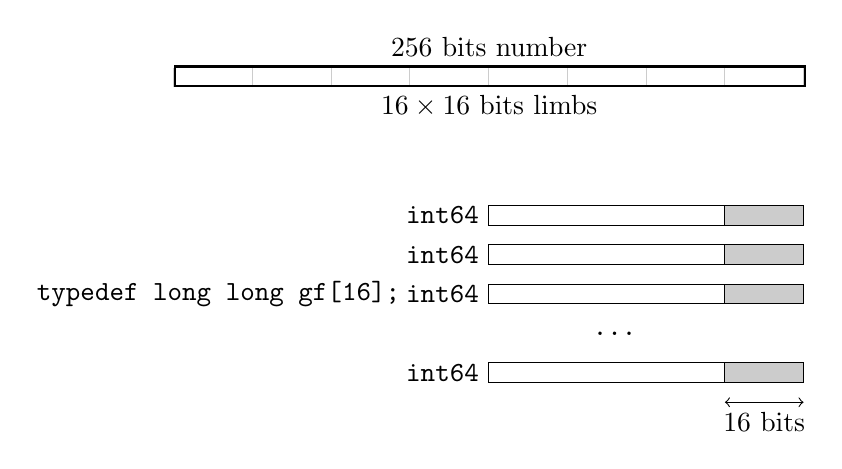
\begin{tikzpicture}[textstyle/.style={black, anchor= south west, align=center}]


  \foreach \x in {0,1,...,8} {
    \draw [black!20] (\x,0) -- (\x,0.25);
  };

  \draw (0,0.25) node[textstyle, minimum width=8cm, minimum height=0.5cm] {$256$ bits number};
  \draw (0,0) node[textstyle, draw=black, thick, minimum width=8cm, minimum height=0.25cm] {};

  \draw (0,-0.5) node[textstyle, minimum width=8cm] {$16 \times 16$ bits limbs};

  \def\yshift{-1.5}
  \def\xshift{4}

  \foreach \y in {0,-0.5,-1,-2} {
    \draw (\xshift+0,\yshift+\y) -- (\xshift+4,\yshift+\y) -- (\xshift+4,\yshift-0.25+\y) -- (\xshift+0,\yshift-0.25+\y) -- cycle;
    \draw [fill=black!20] (\xshift+3,\yshift+\y) -- (\xshift+4,\yshift+\y) -- (\xshift+4,\yshift-0.25+\y) -- (\xshift+3,\yshift-0.25+\y) -- cycle;
    \draw (\xshift,\yshift-0.125+\y) node[anchor= east, align=center] {\texttt{int64}};
  }
  \draw (\xshift+2,\yshift-0.125-1.5) node[anchor= east, align=center] {\texttt{...}};

  \draw (3,\yshift-1.125) node[anchor= east, align=center] {\texttt{typedef long long gf[16];}};

  \def\yshift{-4}
  \draw [<->] (\xshift+3,\yshift) -- (\xshift+4,\yshift);
  \draw (\xshift+3.5,\yshift) node[textstyle, anchor=north] {$16$ bits};



  \end{tikzpicture}

  \end{center}
\end{frame}


%%%%%%%%%%%%%%%%%%%%%%%%%%%%%%%%%
%
%     SLIDE 3
%
%%%%%%%%%%%%%%%%%%%%%%%%%%%%%%%%%
\begin{frame}[fragile]{Basic Operations}
  \begin{center}

\begin{lstlisting}[language=cnacl, caption=Basic Operations, label=cod:languageC31]
#define FOR(i,n) for (i = 0;i < n;++i)
#define sv static void
typedef long long i64;
typedef i64 gf[16];

sv A(gf o,const gf a,const gf b)    # Addition
{
  int i;
  FOR(i,16) o[i]=a[i]+b[i];         # carrying is done separately
}

sv Z(gf o,const gf a,const gf b)    # Zubstraction
{
  int i;
  FOR(i,16) o[i]=a[i]-b[i];         # carrying is done separately
}

sv M(gf o,const gf a,const gf b)    # Multiplication
{
  i64 i,j,t[31];
  FOR(i,31) t[i]=0;
  FOR(i,16) FOR(j,16) t[i+j] = a[i]*b[j];
  FOR(i,15) t[i]+=38*t[i+16];
  FOR(i,16) o[i]=t[i];
  car25519(o);                      # carrying
  car25519(o);                      # carrying
}
\end{lstlisting}

  \end{center}
\end{frame}

\section{From C to Coq}

%%%%%%%%%%%%%%%%%%%%%%%%%%%%%%%%%
%
%     SLIDE 7
%
%%%%%%%%%%%%%%%%%%%%%%%%%%%%%%%%%

\begin{frame}[fragile]{Proving with VST}
  \begin{center}

  \begin{tikzpicture}[textstyle/.style={black, anchor= south west, align=center}]
      \draw (2.75,0) node[textstyle, anchor=west, draw=yellow, fill=yellow!20, thick, minimum width=5.5cm,minimum height=5cm] {};
      \node[inner sep=0pt] (russell) at (5.5,1.5) {
\includegraphics[width=.1\textwidth]{coq_logo.png}};
      \node[inner sep=0pt] (russell) at (5.5,-1.5) {
\includegraphics[width=.15\textwidth]{chain.png}};
      \draw (-1,0) node[textstyle, anchor=east, draw=black, thick, minimum width=1cm,minimum height=2cm] {code.c};
      \draw (0.75,-0.5) node[textstyle, anchor=south] {\texttt{clightgen code.c}};
      \draw (4,0) node[textstyle, anchor=east, draw=black, thick, minimum width=1cm,minimum height=2cm] {code.v};
      \draw (8,0) node[textstyle, anchor=east, draw=black, thick, minimum width=1cm,minimum height=2cm] {proofs.v};
      \node[anchor=west,single arrow,draw=red!80!black,fill=red!80!black,minimum width=0.5cm,minimum height=3.25cm] at (-0.75,0) {};
      \node[anchor=west,double arrow,draw=green!60!black,fill=green!60!black,minimum width=0.5cm,minimum height=2.25cm] at (4.25,0) {};
  \end{tikzpicture}\chapternote{\url{http://vst.cs.princeton.edu}}
  \chapternote{\url{http://compcert.inria.fr}}

  \end{center}
\end{frame}


%%%%%%%%%%%%%%%%%%%%%%%%%%%%%%%%%
%
%     SLIDE 8
%
%%%%%%%%%%%%%%%%%%%%%%%%%%%%%%%%%

\begin{frame}[fragile]{Specification: ZofList}
  \begin{center}
\begin{lstlisting}[language=Coq, caption=ZofList, label=cod:languageC81]
Variable n: \Z.
Hypothesis Hn: n > 0.

(*
  in C we have gf[16] here we consider a list of integers (list \Z)
  of length 16 in this case.

  ZofList convert a list \Z into it's \Z value
  assume a radix: 2^n
*)
Fixpoint ZofList (a : list \Z) : \Z := match a with
| [] => 0
| h :: q => h + 2^n * ZofList q
end.

Notation "\Z.lst A" := (ZofList A) (at level 65).
\end{lstlisting}
  \end{center}
\end{frame}


%%%%%%%%%%%%%%%%%%%%%%%%%%%%%%%%%
%
%     SLIDE 9
%
%%%%%%%%%%%%%%%%%%%%%%%%%%%%%%%%%

\begin{frame}[fragile]{Example: Addition}
  \begin{center}
\begin{lstlisting}[language=Coq, caption=Addition, label=cod:languageC91]
Fixpoint ZsumList (a b : list \Z) : list \Z := match a,b with
| [], q => q
| q,[] => q
| h1::q1,h2::q2 => (Z.add h1 h2) :: ZsumList q1 q2
end.
Notation "A \boxplus B" := (ZsumList A B) (at level 60).

Corollary ZsumList_correct:
  forall (a b: list \Z),
    (\Z.lst a \boxplus b) = (\Z.lst a) + (\Z.lst b).
Qed.

Lemma ZsumList_bound_len:
  forall (m1 n1 m2 n2: \Z) (a b: list \Z),
    length a = length b ->
    Forall (fun x => m1 < x < n1) a ->
    Forall (fun x => m2 < x < n2) b ->
      Forall (fun x => m1 + m2 < x < n1 + n2) (a \boxplus b).
Qed.
\end{lstlisting}

  \end{center}
\end{frame}

% \begin{frame}[fragile]{Example: Addition - Clight}
%   \begin{center}
%     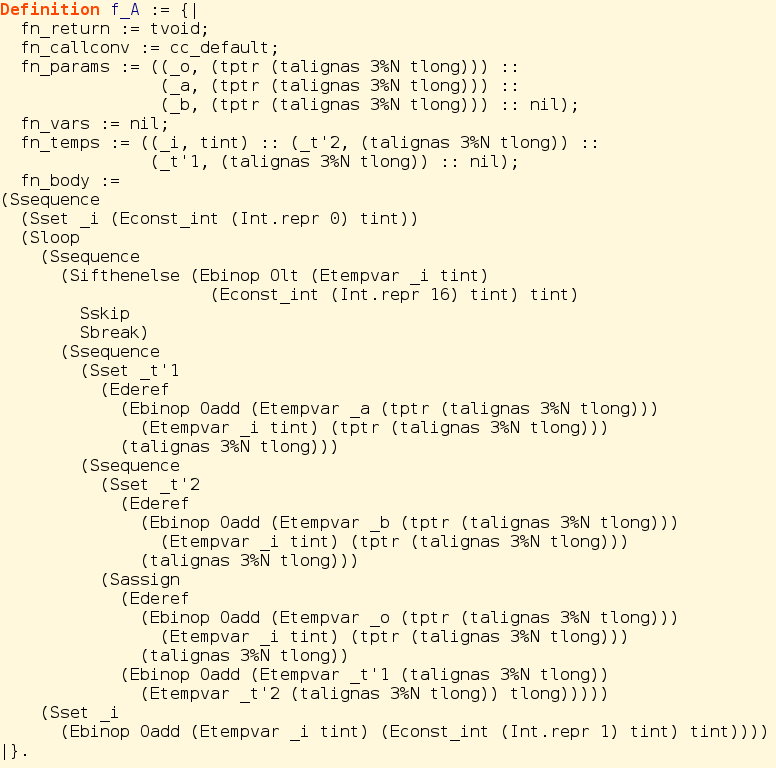
\includegraphics[height=0.8\textheight]{f_A}.
%   \end{center}
% \end{frame}

% \begin{frame}[fragile]{Example: Addition - Spec}
%   \begin{center}
%     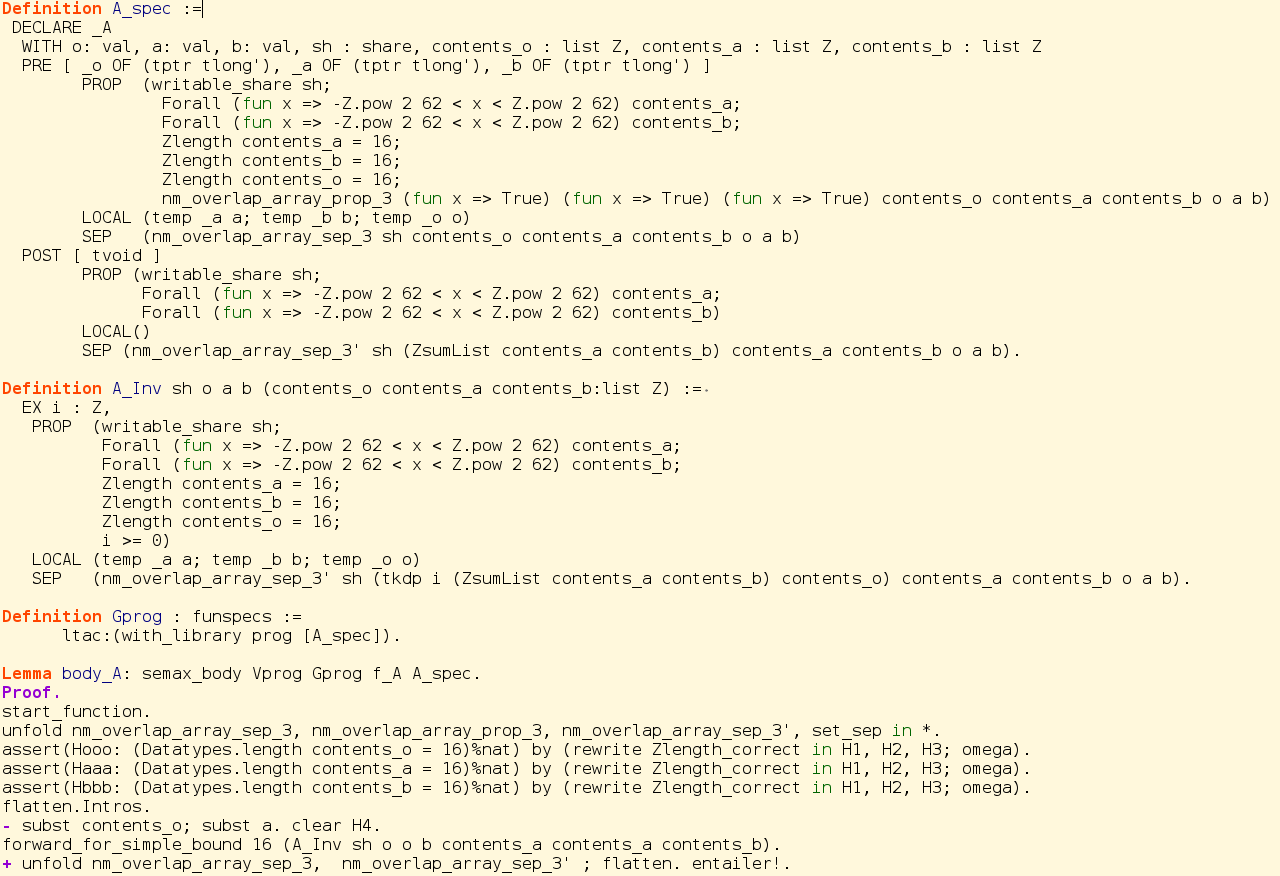
\includegraphics[width=\linewidth]{Spec}.
%   \end{center}
% \end{frame}

\begin{frame}[standout]
  \Huge What's left ?
\end{frame}

\begin{frame}[fragile]{Done so far\ldots}
    \begin{itemize}
      \item[\color{ruDarkTeal}$\blacktriangleright$] Specification of basic operations (A,Z,M,S,Car25519).
      \item[\color{ruDarkTeal}$\blacktriangleright$] Bounds of basic operations.
      \item[\color{ruDarkTeal}$\blacktriangleright$] Proof that model matches the semantic (\texttt{code.v}) using VST 
\includegraphics[height=\fontcharht\font`\B]{princeton-logo}.
    \end{itemize}

    \begin{itemize}
    \item $\sim$10 months.
    \item compiles ({\tt coqc}) in $\sim$1 hours\ldots ({\it i7-4770K CPU @ 3.50GHz})
    \item 62 lines of {\tt C} have been verified.
    \item 7\,180 lines of Specifications with {\tt Coq}.
    \item 2\,872 lines of Verification with {\tt Coq} using VST 
\includegraphics[height=\fontcharht\font`\B]{princeton-logo}.
    \end{itemize}
\end{frame}

\begin{frame}[fragile]{Curent and future Works}
    \begin{itemize}
      \item[\color{ruDarkTeal}$\blacktriangleright$] Proof of a lot of {\it small} utilary functions used in TweetNaCl...
      \item Full Proof of Montgomery Ladder's correctness.
      \item Proof that the model is {\it aligned} with Timmy's work.
      \item Continue on the X25519 signature scheme, Poly1305\ldots
    \end{itemize}
\end{frame}

%%%%%%%%%%%%%%%%%%%%%%%%%%%%%%%%%
%
%     SLIDE 14
%
%%%%%%%%%%%%%%%%%%%%%%%%%%%%%%%%%
\begin{frame}[standout]
	\Huge Thank you.
\end{frame}

\end{document}
